\chapter{Literature Review}
\section{Current Process}
\subsection{Job Descriptions}
\begin{figure}[h]
\centering
\frame{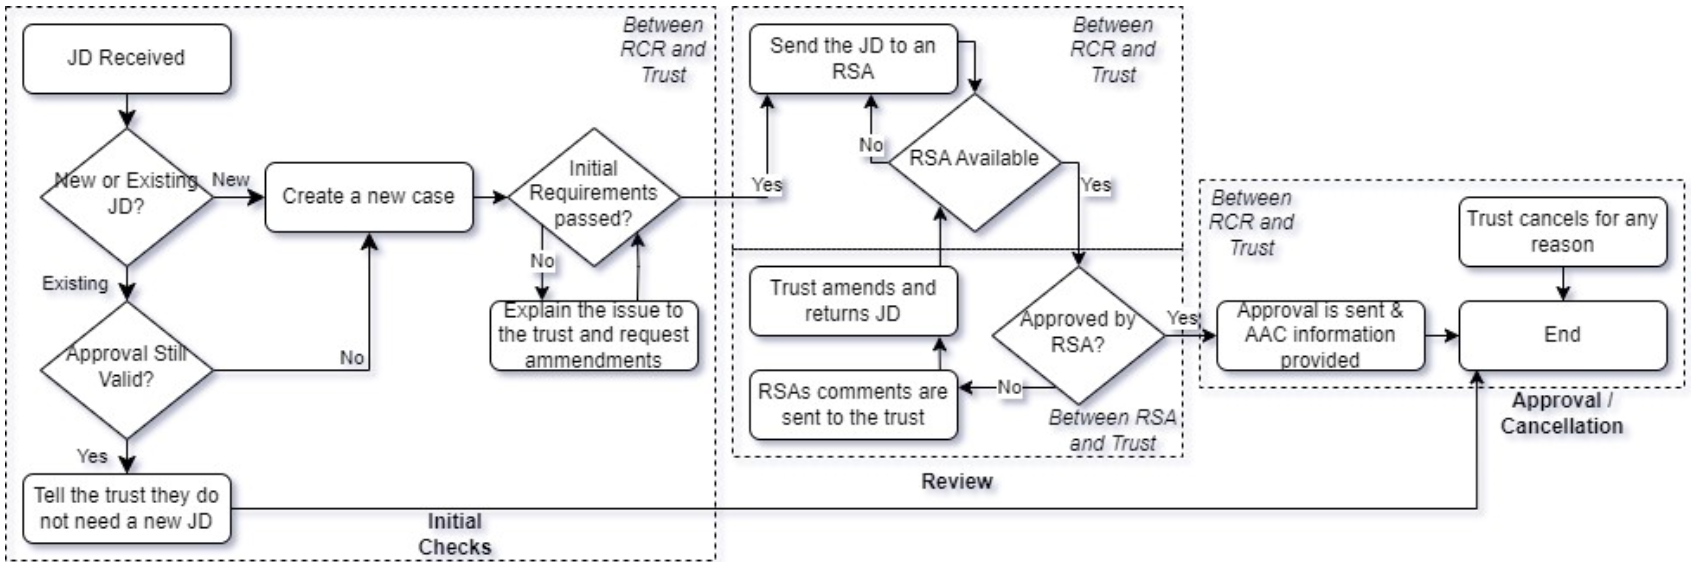
\includegraphics[width=\linewidth]{images/jd.png}}
\vspace{-20pt}
\caption{Job description process}
\label{fig:jd}
\end{figure}
\vspace{-5pt}
The Job Description (JD) process in figure \ref{fig:jd} reflects the meticulous approach followed by the Royal College of Radiologists (RCR) to ensure quality and precision. The process begins with the receipt of a job description, which is then subjected to preliminary checks. If the JD meets the initial criteria, it moves forward to a more detailed examination by a Regional Speciality Advisor (RSA). If the RSA is unavailable at any stage, a new RSA is promptly assigned. The diagram shows multiple checkpoints and potential loops that can occur if information is missing or incomplete, yet every effort must be made to complete this entire process within 2 weeks. The process concludes by informing the Trust that they are permitted to advertise their post and by sending them a form to complete to request a list of representatives.

\subsection{Advisory Appointment Committees}
\begin{figure}[h]
\centering
\frame{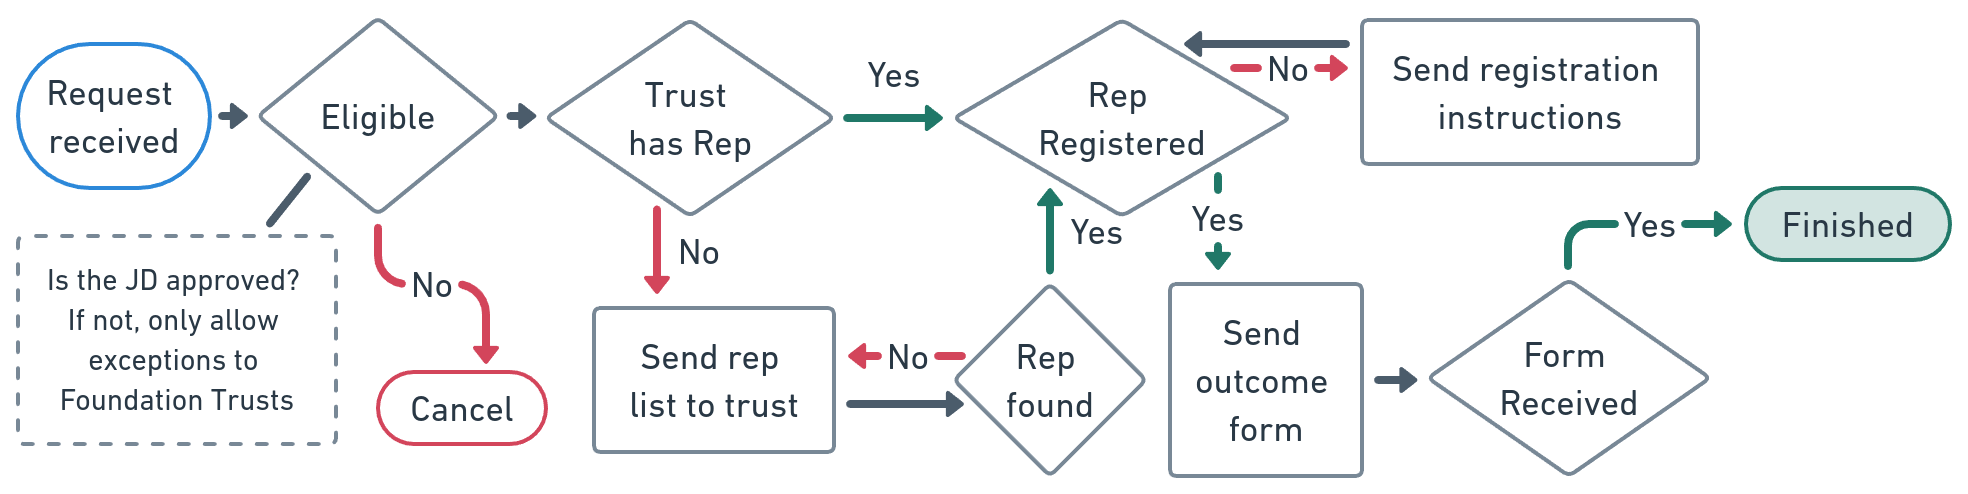
\includegraphics[width=\linewidth]{images/aac.png}}
\vspace{-20pt}
\caption{Advisory appointment committee process}
\label{fig:aac}
\end{figure}
\vspace{-5pt}
The Advisory Appointment Committee (AAC) process in figure \ref{fig:aac} is equally rigorous and focuses on giving Trusts the best chance of securing a representative. This process begins by checking whether the previous Job Description (JD) process was successful, only granting exceptions when requested by a Foundation Trust. Like the JD process, it often involves loops when sending multiple lists to the Trust. If the Trust opts to source their own representative, either upon request or after an unsuccessful search, the appropriate guidance and rules must be sent. All representatives must complete training and registration to attend panels. The process concludes when the representative returns an outcome form sent to them to complete after the panel is held, or if the Trust cancels the panel for any reason.

\section{Related Works}
\subsection{Existing Storage Systems}
With Excel, the primary limitation is the lack of ability to store speciality data. This is because job posts often have multiple primary specialities and secondary sub-specialities. If opting for a single column, data integrity becomes almost impossible as Excel does not inherently support complex data validation for multiple entries within a single cell. This makes it difficult to ensure that the data entered is consistent and makes analysing and querying this data challenging. Using multiple columns for each specialisation provides a more structured way to store this data. However, in this context it quickly becomes unwieldy – in our case we are left with 44 columns. Here the spreadsheet becomes cluttered and difficult to navigate.

The same issues apply to tracking the date of each step of the process, as due to loops in the workflow we often encounter multiple dates in each cell. With no automation whatsoever, these dates, as well as the workflow’s status, must be entered manually every time.

The core issue with both approaches is the lack of normalisation. By splitting data into multiple related tables, and establishing relationships between them, we can reduce redundancy and improve data integrity. This is only realistic if we use a relational database management system like SQL.

\subsection{Healthcare Recruitment Tools}
Searching for software to assist with recruitment in the healthcare sector will bring up results such as \textcite{icims_icims_nodate} and \textcite{the_access_group_access_nodate}. Unfortunately, these programs are typically directed towards the Trust rather than Royal Colleges. Their intended user base is employers looking to advertise and interview candidates, not for those involved in the rigorous job plan review and representative selection process required by the Royal College of Radiologists (RCR). These solutions typically require private meetings, so understanding their capabilities is difficult. For a set of requirements this specific, only personalised software is suitable.

\subsection{Other Royal Colleges}
Finding specific details on the software used by other Royal Colleges in the UK is not possible as this information is not typically disclosed publicly. Though the general process for Advisory Appointment Committees (AAC’s) is somewhat standardised across various Royal Colleges due to the strict requirements set out by the NHS, there is no central piece of software. The advantages to an open-source solution may span beyond just the Royal College of Radiologists (RCR). 

While the overall process is shared, there are still many differences between colleges. Each email and form would differ, and doctors in various departments have distinct needs. A software flexible enough to accommodate everyone is far beyond the scope of this project. For example, the Royal College of Physicians (RCP) requires that medical staffing departments complete the job description review form themselves, in contrast to the RCR filling it out for them. This may, however, be an indication that this project should accommodate any policy changes that the RCR may implement. The RCP also requires foundation Trusts to submit representative requests with a minimum of eight weeks’ notice, a guideline that is optional but recommended in many other colleges, and offers an optional kitemark \parencite{royal_college_of_physicians_of_london_rcp_2017}. Some colleges require the trust to complete the review form for themselves and the reviewer. This is an example of an optimisation to the workflow that could be implemented into the system.

With differing requirements, it’s no wonder that simply sharing software with each other is not a solution. A project that would suit every Royal College would be an expensive undertaking.